% !TEX root=report.tex
\section{Data Exploration}

The CouchSurfing dataset was made privately available to the authors in the form of an anonymized MySQL database dump.
In the course of formulating the prediction problem and our approach to it, we explored and visualized some aspects of the data.

\subsection{Grouping by host and request set.}
Distribution of number of requests received is logarithmic on a logarithmic scale. 
See \autoref{fig:requests_distribution}.

\begin{figure}[ht]
\centering
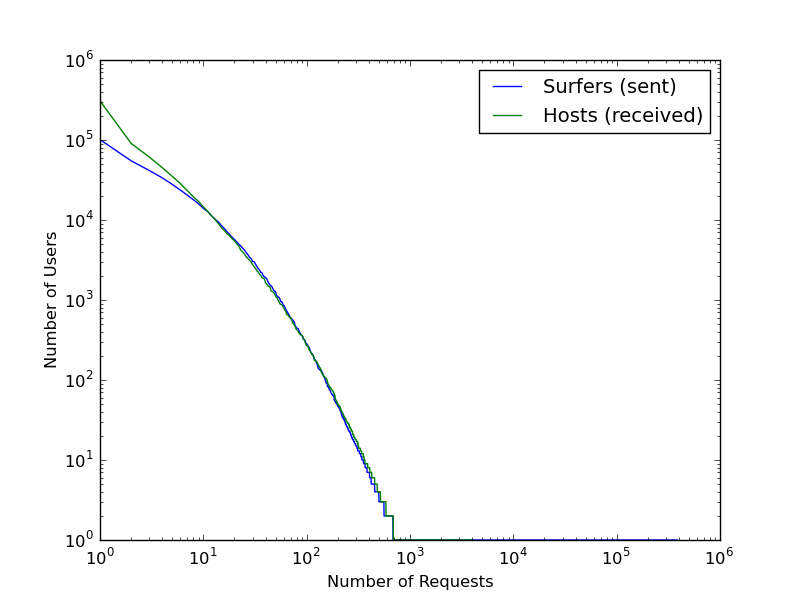
\includegraphics[width=1\linewidth]{figures/req_received_dist2.png}
\caption{Distribution of requests received by a host.}
\label{fig:requests_distribution}
\end{figure}

\subsection{Temporally blind prediction of host-suitor pairings}
The first formulation of the problem ignores the temporal nature of the requests.
We simply wish to answer the prediction problem of which couch requests to a host will result in a match, ignoring any notions of ranking against contemporal requests.

From the CouchSurfing user database, we form a set of \emph{hosts} $\mathcal{H}$ such that every $h \in \mathcal{H}$ has hosted at least $K$ persons since signing up for a user account.
We initially set $K=1$, but the proper setting may be higher to reduce the amount of noise in the set of hosts.

For every host $h_n$, there is a corresponding list of t least $K$ \emph{surfers} $\mathcal{S}_n$, where a suitor $s \in \mathcal{S}_n$ has made at least one couch request to $h_n$.

\subsection{Implicit Negatives}
\label{sec:implicitNeg}
In order to apply learning algorithms to our problem and evaluate the resulting recommendations for the hosts, we need to get positive as well as negative samples from the data. If we just had the positive data (i.e. accepted couches) the only thing we could evaluate for would be \textit{true positives} and \textit{false negatives}, but for a meaningful computation of \textit{precision} and \textit{recall} we also want to learn about \textit{false positives}, which can only be gathered given negative test samples.

In the following, requests carry the same index as the user/suitor that invoked them, i.e., suitor $s_i$ send request $r_{i,j}$ to host $h$. Wlog we can assume for now that each user just sends at most one request to each couch. $h$ is fixed in the upcoming examples, so we just denote requests as $r_i$.
 
The CS system allows hosts to reject a couch request, which indicates a negative sample. We call those \textit{explicit negatives}. Over that it is also possible to imply negatives from other information; If we take for example a host $h$ with a very popular couch in Paris with \note{TB}{reasonable number?}{10s} of requests per day, it is reasonable to assume that $h$ will not look into every request, but will stop reading more requests after deciding for a specific suitor $s_i$. For a given period $\tau$, let $R_{j}^{\tau} = r_1, r_2,\ldots,r_n$ be the requests send to $h$. Assuming that $h$ picks a suitor after reading $k$ requests, we now also have to handle the fact that requests may not be seen at all. Also it might happen that $h$ sees a certain request but decides not to respond to it which is like a negative response. These are called \textit{implicit negatives}. We hereby assume that if at a certain time host $h$ accepts a request $r_i$ for period $\tau$, she prefers the requesting suitor $s_i$ over all other users whose requests she read that overlap with $\tau$. An efficient sweep-line algorithm to find sets of overlapping requests is depicted in \note{TB}{Do we even need this?}{algorithm~\ref{alg:overlap}}. One more important thing to keep in mind is that if $h$ accepted a request for period $\tau$ at time $t_0$ and gets another request $r_l$ for $\tau$ at time $t_1 > t_0$, there is no information about whether or not $h$ likes $s_i$, because his couch is already taken, so we have to filter these out before moving on. Now we observe the positive samples as the accepted requests, explicit and implicit negatives as described above and can evaluate our method.

\begin{algorithm}
\caption{Find overlapping requests}
\label{alg:overlap}
\begin{algorithmic} 
\REQUIRE $R = (r_1, r_2,\ldots,r_n)$, $r_i = (t_i^{start}, t_i^{end})$
\ENSURE $S\subseteq \mathcal{P}(R)$ 
\STATE $S \leftarrow \emptyset$
\STATE $A \leftarrow \emptyset$ 
\STATE $T {(i, start/end, t_i^{s/t}) |r_i \in R}$
\STATE $sort(T, t_i^{s/t})$ 
\STATE $b\_incr \leftarrow True$ 
\FOR{$t$ in $T$}
\IF{$t$ == $v_j^{start}$}
\STATE $A.append(t)$
\STATE $b\_incr \leftarrow True$
\ELSE
\IF{$b\_incr == True$}
\STATE $b\_incr \leftarrow False$
\STATE $S.append({r_i | (i, \_, \_) \in A})$
\ENDIF
\STATE $A.delete(t)$
\ENDIF
\ENDFOR
\end{algorithmic}
\end{algorithm}

It might also be beneficial to soften the notion of ``overlap'' just because it might be very stressful for a host to have surfers without a gap in between the two visits. Analyzing the data for statistics on gaps for each host seperately will reveal their willingness to host several surfers in a row. The above algorithm can easily be adapted by modifying the input times accordingly.

\subsection{Filter rejects by temporal constraints}
Using a very similar technique we can filter rejects that are not actually rejects for the reason of a mismatching suitor. Imagine $h$ gets a request $r_1$ at time $t_1$, accepts this request at time $t_2$ and gets another request $r_2$ for the same period as $r_1$ at $t_3$. If we have that $t_1 < t_2 < t_3$, there is no valid information about whether or not $h$ likes suitor $s_2$. By the time he gets the second request, his couch is already booked out and so he has to reject $s_2$ no matter if he would even prefer him over $s_1$. Because of this scenario we filter our training data for exactly those \textit{uninformative rejects} using again algorithm~\ref{alg:overlap} and temporal orderings on requests and acceptances/rejects.


See \autoref{fig:temporal_filtering}.

\begin{figure}[ht]
\centering
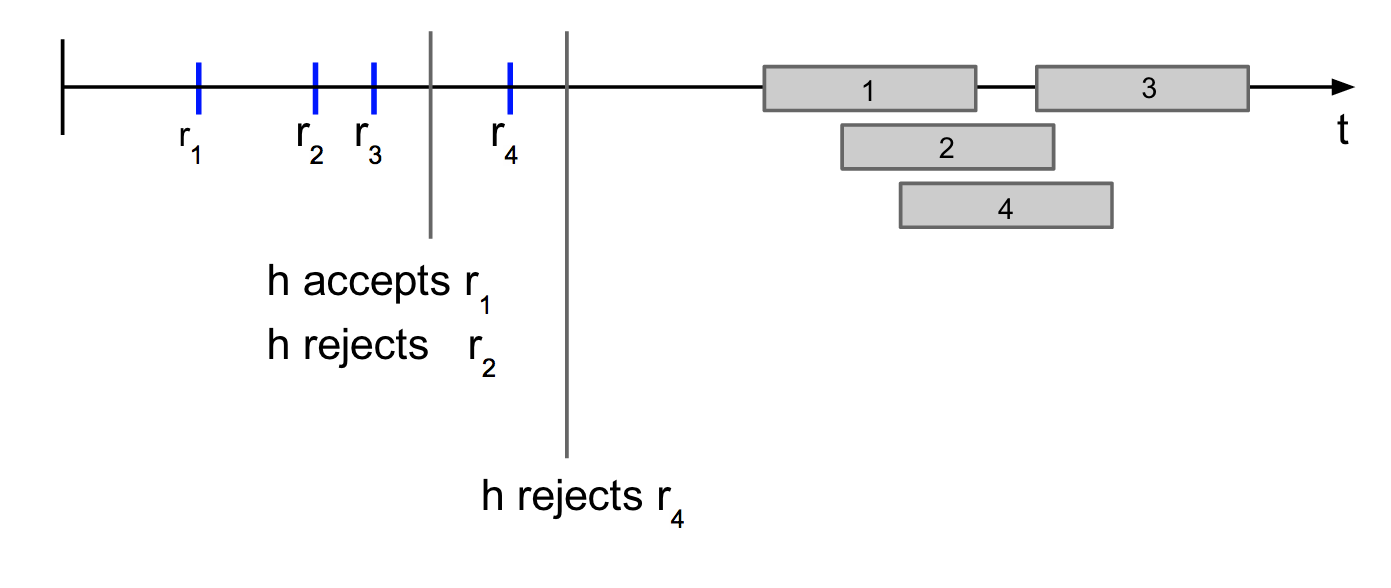
\includegraphics[width=1\linewidth]{figures/temporal_filtering.png}
\caption{Temporal filtering example. \todo{Explain.}}
\label{fig:temporal_filtering}
\end{figure}

\begin{figure}[ht]
\centering
\subfloat[Requested]{
  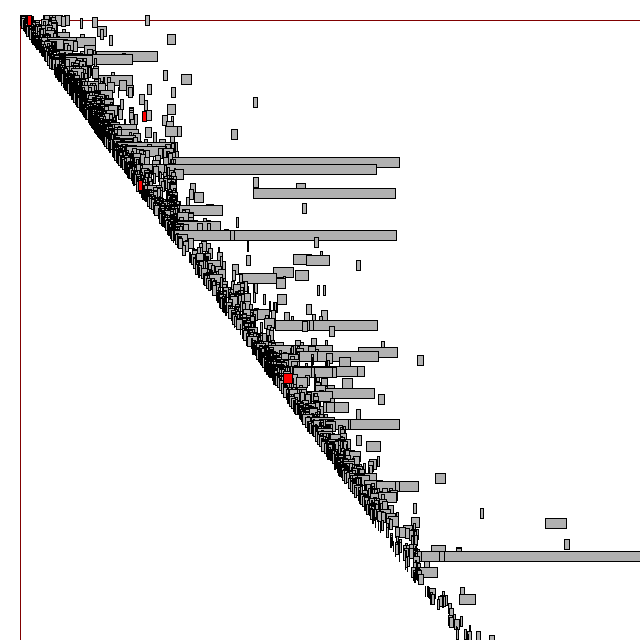
\includegraphics[width=0.45\linewidth]{figures/top_requested.png}
}
\subfloat[Accepted]{
  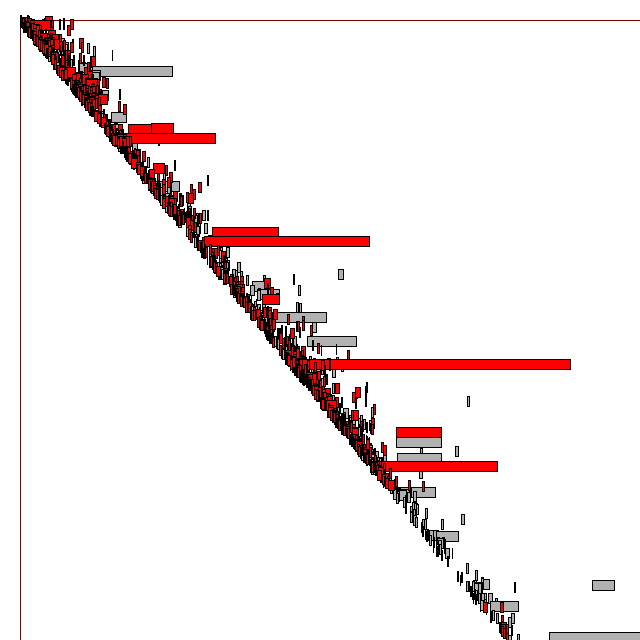
\includegraphics[width=0.45\linewidth]{figures/top_accepted.png}
}
\caption{\todo{Explain.}}
\label{fig:timeline_view}
\end{figure}

\subsection{Unseen Requests}
\label{sec:unseen}
The current state of the system is that $h$ gets an email as soon as a new request is filed and on their profile the requests are presented in \note{TB}{true?}{chronological order} as well. For the mentioned couch in Paris these mails might be archived without being read and interesting request could get lost. For each request $r_i$ we have a binary random variable $seen(h, r_i)$ which is $1$ if $h$ took a look at request $r_i$, independent of whether he click accept/reject/maybe or nothing at all. The probability $p(seen(h,r_i))$ directly corresponds to the objective of this project. The goal is to present the requests to $h$ in order by how likely she is to accept them, or in other words, we want to maximize the probability that $h$ \textit{sees} requests that she would accept by moving them upwards in our ranking and hence reducing the number of overall requests to look at. Maximizing the acceptance/\#views rate is the same as minimizing the rejection/\#views rate, which can be expressed as finding a permutation $\sigma^*$, such that:
$$\sigma^* = \arg\min_{\sigma}\sum_{i=1}^k p(reject(h, r_{\sigma_i}))$$
where $k$ is the number of requests that are shown to $h$. 
In section~\ref{sec:implicitNeg} we assumed that all requests in the \textit{implicit negatives} have been seen by $h$, which is not a perfectly valid model as just stated. Instead we have to compute the following:
$$p(reject(h, r_i)) = \int p(reject(h, r_i)|seen(h, r_i))\cdot p(seen(h, s_i))$$
To do so we need a way to estimate $p(seen(h,s_i))$. This probability is both dependent on the manner of $h$ as well as on the order of how the requests are shown to $h$, which is dependent on the time $h$ looks at the requests. We do not have log-files of the website, so we cannot determine which requests $h$ has acutally seen, but we can again try to infer this information from the behavior of the host. Assuming that $h$ acts during each visit of her request-list at least once with a click onto accept/reject/maybe (\textit{active visit}), we can interpolate for each of these events the request-list she saw and assume that $h$ looked at the first $l$ of these requests. We can now for each \textit{active visit} sum up the number of requests $h$ actually saw and reacted upon and the discounted number of the first $l$ request in the list, discounted by $\lambda_i$ for their position $i$ in the list as well as with another host-specific factor $\lambda$.

\subsection{User interests}
Interest graph: the compatibility strength between suitor and host is determined by $num_overlapping_interest(host, suitor)$ through some type of decaying activation propagation.  This will be based on the "Taste Fabric" paper and the "Semantic Recommendation" paper.  This method assumes homophily and that interests are the strongest attractors between people (doesn't take into account demographics etc.).  This method is reversible.

\begin{figure}[ht]
\centering
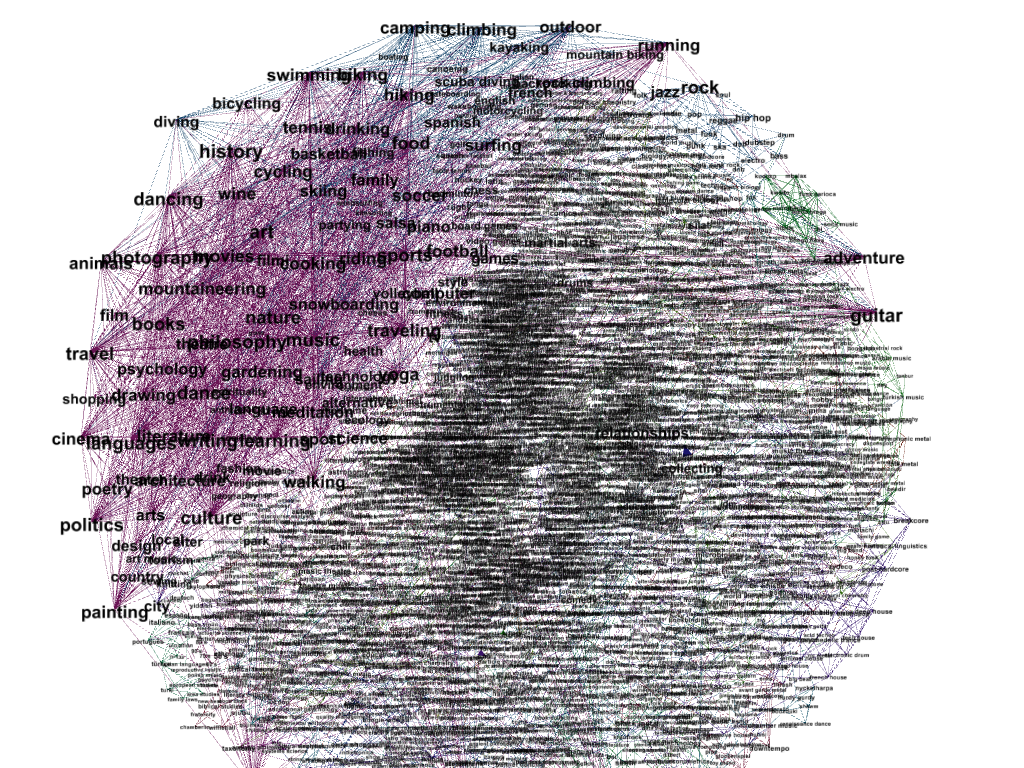
\includegraphics[width=1\linewidth]{figures/interest_graph.png}
\caption{Interest graph.}
\label{fig:interest_graph}
\end{figure}
